%&LaTeX
\documentclass{article}
\usepackage{graphicx}
\usepackage{longtable}

\oddsidemargin 0.5in    %   Note that \oddsidemargin = \evensidemargin
\evensidemargin 0.5in
\marginparwidth 40pt      
\marginparsep 20pt      % Horizontal space between outer margin and
                % marginal note
\textwidth 5.5in        % width of text

% VERTICAL SPACING:
% Top of page:
%\topmargin .5in     %    distance from top of page to running head
\headheight 14pt     %    Height of box containing running head.
\headsep .4in        %    Space between running head and text.
\textheight 8.8in    %    space for text
\footskip 30pt       %    Distance from baseline of box containing foot
             %    to baseline of last line of text.
                                                  
\begin{document}

\hspace{-1in}
\includegraphics[height=8.5in, width=7.3in]{figures/iBase.eps}

\newpage
\tableofcontents
\newpage
%%%%%%%%%%%%%%%%%%%%%%%%%%%%%%%%%%%%%%%%%%%%%%%%%%%%%%%%%%
%%%%%%%%%%%%%%%%%%%%%%%%%%%%%%%%%%%%%%%%%%%%%%%%%%%%%%%%%%
\section{Introduction: Interoperability and Interchangeablity}
%%%%%%%%%%%%%%%%%%%%%%%%%%%%%%%%%%%%%%%%%%%%%%%%%%%%%%%%%%
%%%%%%%%%%%%%%%%%%%%%%%%%%%%%%%%%%%%%%%%%%%%%%%%%%%%%%%%%%

One of the primary goals of the Terascale Simulation Tools and 
Technologies (ITAPS) center is to provide an array of advanced 
meshing and discretization services to application scientists. 
These can range from mesh-based services such as mesh quality 
improvement and adaptive loop insertion to field data services 
such as high-order discretization libraries and simulation coupling 
approaches for multiscale and multiphysics applications. Ideally 
these services will be both \textit{interchangeable}, allowing experimentation 
horizontally across a number of different tools that provide 
similar functionality, and \textit{interoperable}, allowing vertical 
integration of multiple tools into a single simulation. Unfortunately, 
most modern meshing and discretization technologies are not interchangeable 
or interoperable making it difficult and time consuming for an 
application scientist to pursue a number of advanced solution 
strategies. 

\begin{figure}[htbp]
\begin{center}
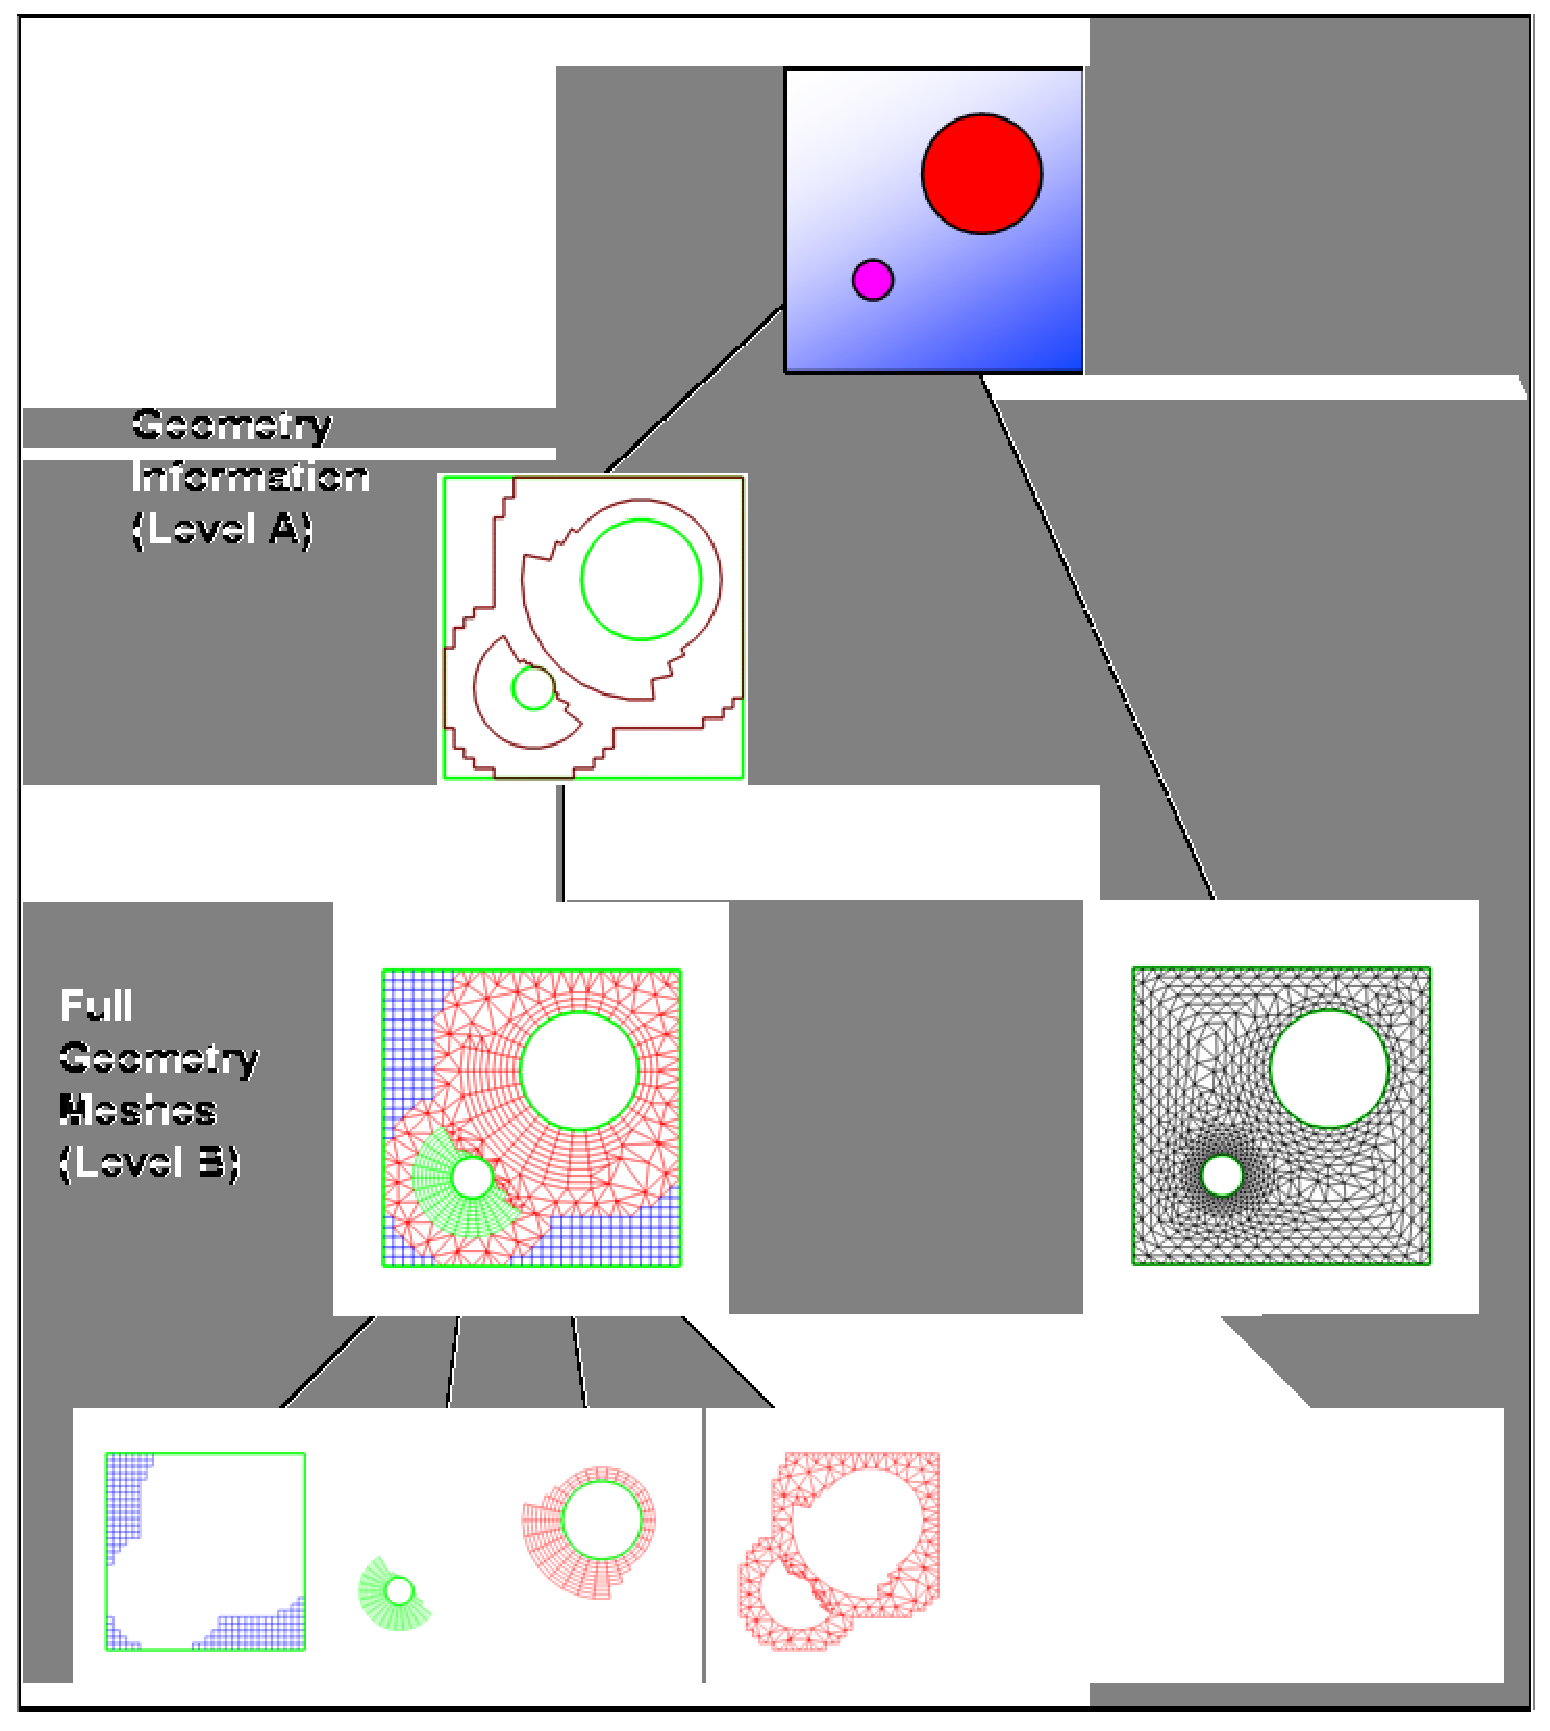
\includegraphics[bb = 0 0 728 815, scale=0.23]{figures/iBase-fig1.eps}
\caption{The abstract data hierarchy for PDE-based 
simulations}\label{fig1}
\end{center}
\end{figure}

To create a set of interoperable and interchangeable services, 
the ITAPS center has defined a framework that abstracts the information 
flow in PDE-based simulations and this is shown in Figure~\ref{fig1}. 
A simulation's information flow 
begins with a problem definition. Described in more detail in 
the iGeom users' guide, the problem definition consists of a 
description of the simulation's geometric and temporal domain 
annotated by attributes designating mathematical model details 
and parameters. The description of the computational domain which 
can take one of many different forms including CAD models, image 
data, or a surface mesh. We note that the geometry can be decomposed 
into one or more subpieces if a multiphysics solution is to be 
pursued in which different mesh types or physics models are desired 
for different parts of the domain. In the next stage of the information 
flow, mesh-based simulation procedures approximate the PDEs by 
first decomposing the geometric domain into a set of piecewise 
components, \textit{the mesh}, and then approximating the continuous 
PDEs on that mesh using, for example, finite difference, finite 
volume, finite element, or partition of unity methods. These 
may be single meshes with a consistent element type or hybrid 
meshes in which multiple meshing strategies have been employed. 
All meshes at this level refer back to a single high level description 
of the computational domain (even if it has been decomposed) 
so that changes to the computational domain propagate throughout 
all associated simulation processes. The mesh can be further 
subdivided, perhaps into the components of a hybrid mesh or partitions 
across the processors of a parallel computer. In addition to 
the mesh and geometry data, the third core data type in the ITAPS 
data hierarchy is the field data or degrees of freedom used in 
the numerical solution of PDE-based applications. Once the domain 
and PDE are discretized, a number of different methods can be 
used to solve the discrete equations and visualize or otherwise 
interrogate the results. Simulation automation and reliability 
often imply feedback of the PDE discretization information back 
to the domain discretization (i.e. in adaptive methods) or even 
modification of the physical domain or attributes (e.g., design 
optimization). ITAPS uses the information flow through a mesh-based 
simulation as a framework for developing interoperable geometry, 
mesh and solution field components. While the information flow 
is modeled using the requirements of a mesh-based PDE solver, 
the resulting components are general enough to provide the infrastructure 
for a variety of other tools including pre/post-processing of 
discrete data, mesh and geometry manipulation, and error estimation.

\begin{figure}[htbp]
\begin{center}
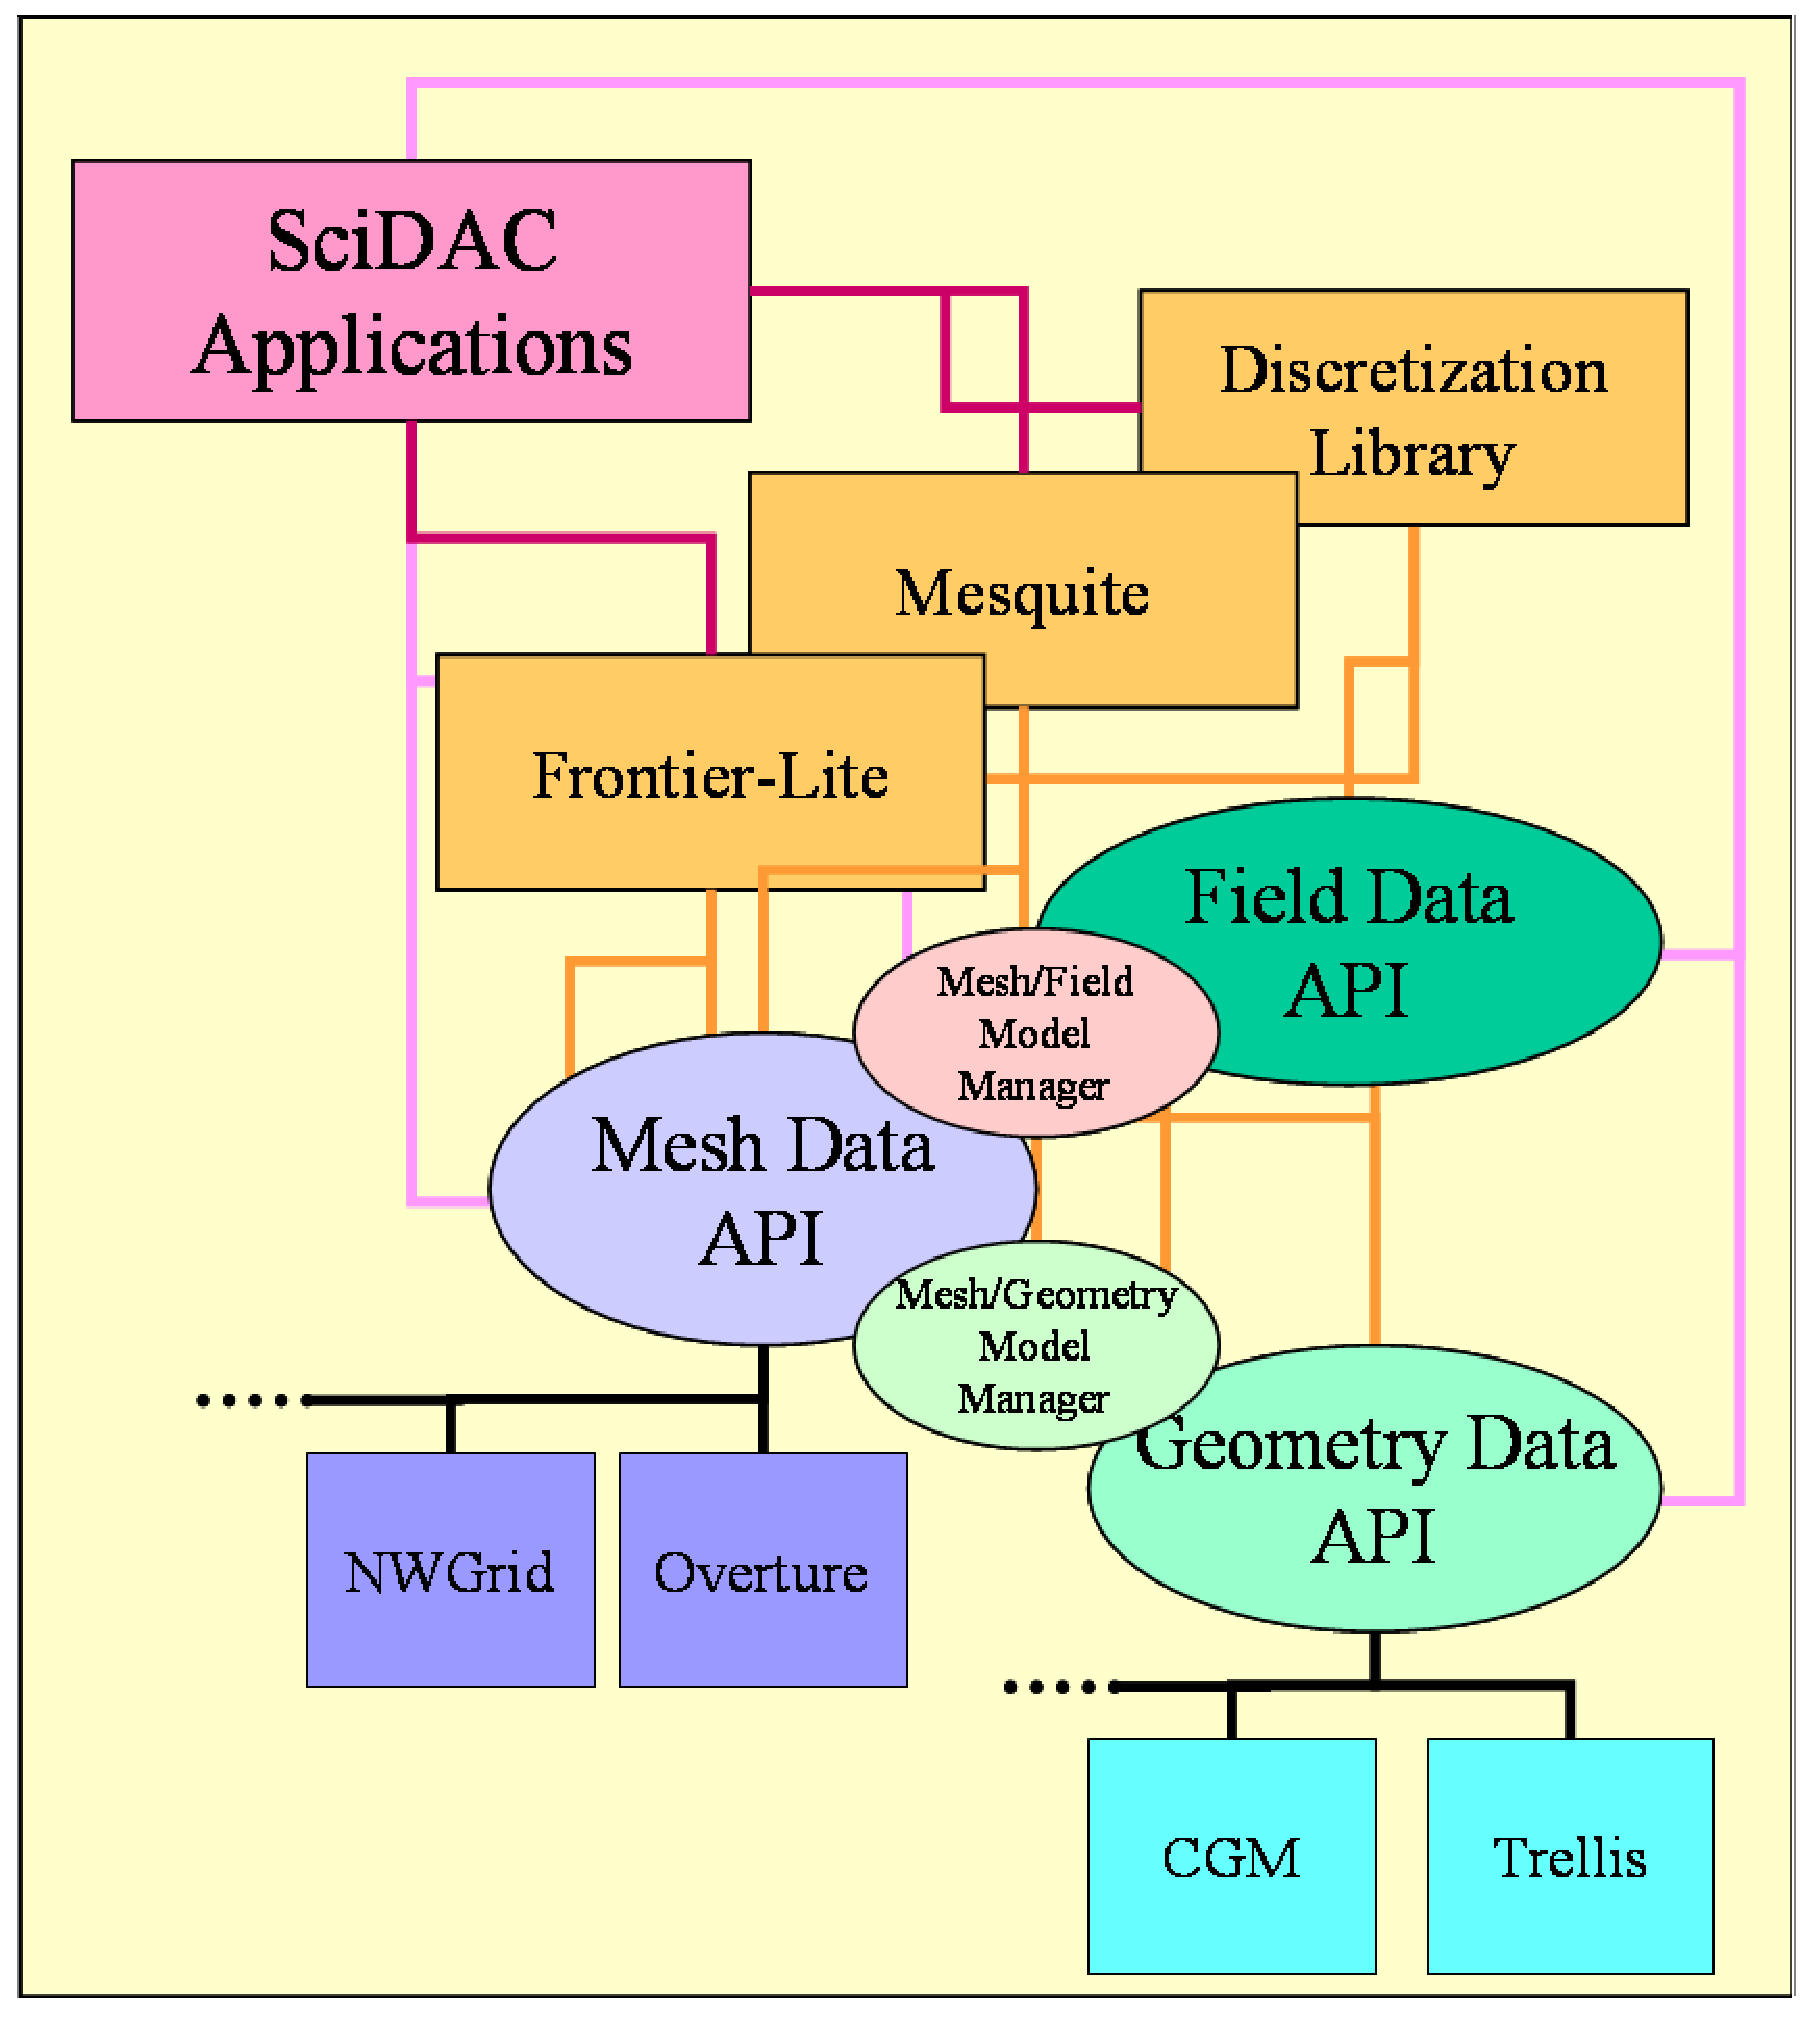
\includegraphics[bb = 0 0 853 953, scale=0.20]{figures/iBase-fig2.eps}
\caption{The ITAPS interoperability plan}\label{fig2}
\end{center}
\end{figure}

Given the data hierarchy framework defined above, researchers 
in the ITAPS center are working along multiple fronts to achieve 
interoperable and interchangeable meshing and discretization 
technology. Figure \ref{fig2} shows a schematic of the ITAPS center plan 
for technology development. The boxes in orange highlight a number 
of example ITAPS services, namely an interface- or front-tracking 
library based on the Frontier-Lite software, mesh quality improvement 
services in the Mesquite toolkit, and a number of high-order 
discretization schemes in the ITAPS discretization library. To 
be interoperable with a number of different meshing packages, 
these services will use a set of ITAPS-defined common interfaces 
for meshes, geometries, and fields. These interfaces have been 
designed by a large number of participants and will wrap existing 
mesh and geometry tools such as FMDB (RPI), GRUMMP (UBC), MOAB 
(SNL), NWGrid (PNNL), and Overture (LLNL). Each of these implementations 
provides a number of services in and of themselves and can be 
used with any of the ITAPS services. Existing applications may 
use any of the ITAPS services by providing the necessary ITAPS 
function calls as wrappers around their mesh, geometry, and field 
data structures. As new applications are developed it is often 
unclear a priori which meshing and discretization strategy is 
best for a particular simulation. By using the ITAPS interface, 
it is easy to experiment with the broad range of ITAPS technologies 
to determine which method is best suited for a given application's 
needs.\\



A key aspect of our approach is that we do not enforce any particular 
data structure or implementation with our interfaces, only that 
certain questions about the mesh, geometry or field data can 
be answered through calls to the interface. The challenges inherent 
in this type of effort include balancing performance of the interface 
with the flexibility needed to support a wide variety of mesh 
types. Further challenges arise when considering the support 
of many different scientific programming languages. This aspect 
is addressed through our joint work with the Center for Component 
Technologies for Terascale Simulation Science (CCTTSS) to provide 
language independent interfaces by using their SIDL/Babel technology. \\

This document focuses on the definition of the functional interface 
for ITAPS data model concepts that are common across the mesh, 
geometry and field interfaces, in particular the concepts of 
entities, entity sets and tags. Documentation on the use of these 
concepts in the mesh, geometry and field data interfaces can 
be found in separate documents. The remainder of this users' 
guide is organized as follows. We discuss basic concepts behind 
the ITAPS data model in Section 2, and the assumptions and conventions 
used in the interface definition process in Section 3. A functional 
description of the tag and entity set interfaces is given in 
Sections 4 and 5. 

%%%%%%%%%%%%%%%%%%%%%%%%%%%%%%%%%%%%%%%%%%%%%%%%%%%%%%%%%%
%%%%%%%%%%%%%%%%%%%%%%%%%%%%%%%%%%%%%%%%%%%%%%%%%%%%%%%%%%
\section{ITAPS Data Model Concepts}
%%%%%%%%%%%%%%%%%%%%%%%%%%%%%%%%%%%%%%%%%%%%%%%%%%%%%%%%%%
%%%%%%%%%%%%%%%%%%%%%%%%%%%%%%%%%%%%%%%%%%%%%%%%%%%%%%%%%%

The ITAPS data models for mesh, geometry and fields all make use 
of the concepts of \textit{entities}, \textit{entity sets}, and \textit{tags}, 
and we describe these now in some detail.\\

ITAPS \textit{entities} are used to represent atomic pieces of information 
such as vertices in a mesh or edges in a geometric model. To 
allow the interface to remain data structure neutral, entities 
(as well as entity sets and tags) are uniquely represented by 
opaque handles. Unless entities are added to or removed, these 
handles must be invariant through different calls to the interface 
in the lifetime of the ITAPS interface, in the sense that a given 
entity will always have the same handle. Entities do not have 
interface functionality that is separate from mesh, geometry 
or field interfaces, which we describe these functionalities 
in detail in the relevant user guides.\\


A ITAPS \textit{entity set} is an arbitrary collection of ITAPS entities 
that have uniquely defined entity handles. Each entity set may 
be an unordered set or it may be a (possibly non-unique) ordered 
list of entities. When a ITAPS interface is first created in a 
simulation, a \textit{Root Set} is created to which all entities and 
entity sets associated with that interface belong. In addition 
to containing entities, entity sets may be related to each other 
in one of two ways.


\begin{itemize}
\item Entity sets may \textit{contain} one or more entity sets. An entity 
set contained in another may be either a subset or an element 
of that entity set. The choice between these two interpretations 
is left to the application; ITAPS supports both interpretations. 
If entity set $A$ is contained in entity set $B$, a request for the 
contents of $B$ will include the entities in $A$ and the entities 
in sets contained in $A$ if the application requests the contents 
recursively. We note that the \textit{Root Set} cannot be contained 
in another entity set.

\item \textit{Parent/child relationships} between entity sets are used to 
represent relations between sets, much like directed edges connecting 
nodes in a graph. This relationship can be used to indicate that 
two meshes have a logical relationship to each other, including 
multigrid and adaptive mesh sequences. Because we distinguish 
between parent and child links, this is a directed graph. Also, 
the meaning of cyclic parent/child relationships is dubious, 
at best, so graphs must be acyclic. No other assumptions are 
made about the graph.
\end{itemize}

Users are able to query entity sets for their entities and entity 
adjacency relationships. Both array- and iterator-based access 
patterns are supported. In addition, entity sets also have Boolean 
set operation capabilities; in particular, existing ITAPS entities 
may be added to or removed from the entity set, and sets may 
be subtracted, intersected, or united. \\

ITAPS \textit{tags} are used as containers for user-defined opaque 
data that can be attached to ITAPS entities and entity sets. Tags 
can be multi-valued which implies that a given tag handle can 
be associated with many different entities and, potentially, 
have a different value on each entity (for example, a tag that 
stores spatially varying boundary condition or material property). 
In the general case, ITAPS tags do not have a predefined type 
and allow the user to attach any opaque data to ITAPS entities. 
 To improve performance and ease of use, we support three specialized 
tag types: integers, doubles, and entity handles. Tags have and 
can return their string name, size, handle and data. Tag data 
can be retrieved from ITAPS entities by handle in an agglomerated 
or individual manner. The ITAPS implementation is expected to 
allocate the memory as needed to store the tag data. As an example, 
a tag may be created to store a material property value on a 
subset of mesh entities. \\

The functionality associated with tags and entity sets that is 
not specific to their relationship with the mesh, geometry or 
field interface are defined in the iBase interface file. Interface 
specific functions are defined in the appropriate interface documents 
(iMesh, iGeom, or iField).


%%%%%%%%%%%%%%%%%%%%%%%%%%%%%%%%%%%%%%%%%%%%%%%%%%%%%%%%%%
%%%%%%%%%%%%%%%%%%%%%%%%%%%%%%%%%%%%%%%%%%%%%%%%%%%%%%%%%%
\section{Interface Definition Conventions}
%%%%%%%%%%%%%%%%%%%%%%%%%%%%%%%%%%%%%%%%%%%%%%%%%%%%%%%%%%
%%%%%%%%%%%%%%%%%%%%%%%%%%%%%%%%%%%%%%%%%%%%%%%%%%%%%%%%%%

In this document, we use \textit{application} to indicate a code that 
will use the ITAPS interface, and \textit{implementation} to indicate 
a code that provides all or part of the ITAPS interface functionality.


%%%%%%%%%%%%%%%%%%%%%%%%%%%%%%%%%%%%%%%%%%%%%%%%%%%%%%%%%%
\subsection{Scientific Interface Definition Language}
%%%%%%%%%%%%%%%%%%%%%%%%%%%%%%%%%%%%%%%%%%%%%%%%%%%%%%%%%%

In the interfaces presented in this document we use the Scientific 
Interface Definition Language (SIDL) to define the functions. 
Each argument in the SIDL interface specification has both a 
type and a mode associated with it. We extensively use SIDL's 
fundamental types including bool, int, double, string, opaque, 
and enumerations.\footnote{{\small We do not use objects due to the perceived 
cost of object creation and access at a fine grained level such 
as mesh entity by entity access. To validate this design choice, 
experiments are underway involving the ITAPS and Babel teams to 
quantify the performance differences among language specific 
bindings, SIDL bindings with opaques, and SIDL bindings with 
objects.} }\\

Argument modes can be one of \textit{in, out} or \textit{inout.} In general, 
SIDL defines \textit{in} to be a parameter that is passed into the 
implementation (but is not necessarily a const), \textit{out} to be 
parameters that are passed out of the implementation, and \textit{inout} 
to be parameters that do both. For ITAPS purposes, we expect the 
following, more restrictive behavior to be associated with implementations
\begin{itemize}
\item \textit{in}: the parameter is passed into the implementation. It is 
guaranteed that any variable passed as an `in' argument will not 
be modified within the function call, even if a particular language 
implements the function call using pass-by-reference semantics. 
\item \textit{out}: the parameter is passed out of the implementation and 
is not expected to contain meaningful data upon entering. The 
underlying implementation is free to operate as needed to allocate 
the necessary space and assign a meaningful value.
\item \textit{inout:} the parameter is passed into the implementation 
and may or may not contain useful information upon entering the 
function. Its value can be changed by the underlying implementation. 
Arrays declared to be inout typically have `out' semantics. That 
is any values originally contained in the array are often overwritten 
by the underlying implementation but it is passed as inout so 
storage in the array can be allocated during the function call.
\end{itemize}

We use SIDL arrays and have the following general expectations 
of the interactions of the application and the implementation 
for their use as \textit{inout} arguments.
\begin{itemize} 
\item The application must allocate sufficient space in the array or 
pass an empty, unallocated array
\item If the passed array is unallocated, the implementation will allocate 
sufficient space in the array
\item If the passed array is allocated, the implementation will indicate 
an error condition if the allocated space is not sufficient for 
the requested data.
\item If the passed array is allocated, it must be allocated as a 1-dimenstional 
array (a vector)
\item If the particular language requires an explicit call to release 
the array storage, it is the responsibility of the caller to 
do so regardless of whether or not the storage was allocated 
within the function.
\end{itemize}


Functions that work with arrays that contain a set of fixed-length 
vectors of data (such as vertex coordinate triples) may accept 
or return such arrays ordered in either an interleaved or blocked 
manner. The application may request either order, and the implementation 
is expected to be able to provide both. It is recognized that 
the implementation may have a preferred, native storage order 
and this preferred ordering may be queried by the application.


%%%%%%%%%%%%%%%%%%%%%%%%%%%%%%%%%%%%%%%%%%%%%%%%%%%%%%%%%%
\subsection{Function Naming Conventions}
%%%%%%%%%%%%%%%%%%%%%%%%%%%%%%%%%%%%%%%%%%%%%%%%%%%%%%%%%%

ITAPS interfaces have the following naming conventions:
\begin{itemize}
\item As much as possible, functions start with a verb describing the 
action of the implementation, for example, \textit{get, set, create, 
destroy.}

\item To provide maximum flexibility for achieving performance, we 
have defined interfaces that allow access of information for 
either individual entities (\textit{single entity access)} or for 
several entities agglomerated into an array (\textit{agglomerated 
entity access)}. Functions that operate on individual entities 
contain ``Ent'' in the function name; functions that operated 
on arrays of entities contain ``Arr'' or ``EntArr''

\item Function arguments that contain the word ``handle'' are 
opaque references to underlying implementation data structures. 
The application should not make any assumptions about the specific 
value of the handle.

\item Members of enumerated types are given in capital letters
\end{itemize}

To accommodate the 31-character limit imposed by some Fortran 
compilers we have used the following abbreviations in the function 
names

\begin{itemize}
\item {\tt Coords} for coordinates
\item {\tt Vtx} for vertex
\item {\tt Ent} for entity
\item {\tt Arr} for array
\item {\tt Adj} for adjacency
\item {\tt Dim} for dimension
\item {\tt Dflt} for default
\item {\tt Topo} for topology
\item {\tt Num} for number
\item {\tt Init} for initialize
\item {\tt Iter} for iterator
\item {\tt Chldn} for children ({\tt chld} for child)
\item {\tt Prnts} for parents ({\tt prnt} for parent)
\item {\tt Rmv} for remove
\item {\tt Int} for integer
\item {\tt Dbl} for double
\item {\tt EH} for entity handle
\end{itemize}

%%%%%%%%%%%%%%%%%%%%%%%%%%%%%%%%%%%%%%%%%%%%%%%%%%%%%%%%%%
%%%%%%%%%%%%%%%%%%%%%%%%%%%%%%%%%%%%%%%%%%%%%%%%%%%%%%%%%%
\section{ITAPS Tags}
%%%%%%%%%%%%%%%%%%%%%%%%%%%%%%%%%%%%%%%%%%%%%%%%%%%%%%%%%%
%%%%%%%%%%%%%%%%%%%%%%%%%%%%%%%%%%%%%%%%%%%%%%%%%%%%%%%%%%

Tags are used as containers for user-defined opaque data that 
can be attached to ITAPS entities and entity sets. Tags can be 
multi-valued which implies that a given tag handle can be associated 
with many entities.

%%%%%%%%%%%%%%%%%%%%%%%%%%%%%%%%%%%%%%%%%%%%%%%%%%%%%%%%%%
\subsection{Tag Types}
%%%%%%%%%%%%%%%%%%%%%%%%%%%%%%%%%%%%%%%%%%%%%%%%%%%%%%%%%%
In the general case, ITAPS tags do not have a predefined type 
and allow the user to attach any opaque data to mesh entities. 
To improve ease of use and performance, we support three specialized 
tag types: integers, doubles, and entity handles. The tag value 
bytes is used for the general case. If a specialized tag type 
is used, it is set during tag creation using a data type specific 
function. When retrieving specialized tag data, data specific 
functions are available. The tag types are given in the enumerated 
type
\begin{verbatim}
    enum TagValueType { 
        INTEGER, 
        DOUBLE, 
        ENTITY_HANDLE, 
        BYTES 
    };
\end{verbatim}

%%%%%%%%%%%%%%%%%%%%%%%%%%%%%%%%%%%%%%%%%%%%%%%%%%%%%%%%%%
\subsection{Basic Tag Functionality}
%%%%%%%%%%%%%%%%%%%%%%%%%%%%%%%%%%%%%%%%%%%%%%%%%%%%%%%%%%
Create a tag with specified string name, tag 
type, and number of values of that tag type, and return the associated 
tag handle. Tag data may be a vector of the specified type and 
is specified by indicating a number of values greater than 1. 
The tag name is a unique string; if it duplicates an existing 
tag name, an error is returned. The {\tt tag\_handle} is returned as 
an opaque value which is not associated with any entities until 
explicitly done so through one of the `setTag' functions defined 
later. The implementation is assumed to allocate memory as needed 
to store the tag data.

\begin{verbatim}
    void createTag( in string tag_name, in int number_of_values, 
                    in TagValueType tag_type,
                    out opaque tag_handle) throws Error;
\end{verbatim}

Delete a tag handle and the data associated with that tag. The 
deletion can be forced or not forced. If the deletion is forced, 
the tag and all of its associated data are deleted from the implementation 
even if the tag is still associated with mesh entities. If the 
deletion is not forced, the tag will not be deleted if it is 
still associated with one or more mesh entities. In this case 
an error is returned asking the user to remove the tag from that 
entity before deleting it.  If the underlying implementation 
does not support the requested deletion mechanism, an error will 
be returned.

\begin{verbatim}
    void destroyTag( in opaque tag_handle, in bool forced) throws Error;
\end{verbatim}

Get the tag name associated with a given tag handle.
\begin{verbatim}
    string getTagName( in opaque tag_handle) throws Error;
\end{verbatim}

Get the number of values of {\tt tag\_type} associated with a given 
tag handle.
\begin{verbatim}    
    int getTagSizeValues( in opaque tag_handle) throws Error;
\end{verbatim}

Get the total size of the tag data in bytes associated with a 
given tag handle.
\begin{verbatim} 
    int getTagSizeBytes ( in opaque tag_handle) throws Error;
\end{verbatim}

Get the tag data type associated with a given tag handle.
\begin{verbatim} 
    TagValueType getTagType( in opaque tag_handle) throws Error;
\end{verbatim}

Get the tag handle associated with a given string name.
\begin{verbatim} 
    opaque getTagHandle( in string tag_name) throws Error;
\end{verbatim}

%%%%%%%%%%%%%%%%%%%%%%%%%%%%%%%%%%%%%%%%%%%%%%%%%%%%%%%%%%
\subsection{Using Tags}
%%%%%%%%%%%%%%%%%%%%%%%%%%%%%%%%%%%%%%%%%%%%%%%%%%%%%%%%%%

The user can set tag data values on an entity or an array of 
entities. The tag is identified by a tag handle created using 
the tagCreate function. If the tag is not already associated 
with the entity, the association is created and the tag value 
is set. Otherwise, the tag value is changed. All entity tag values 
associated with a particular tag handle by various setData calls 
are accessed through the same tag handle.\\


Allows the user to set the tag data values on a single entity. To 
allow opaque tags of various sizes to be used in the ITAPS interface 
we pass in the value as array of characters (1 byte each). The 
{\tt tag\_value\_size} argument must be the number of values associated 
with the tag data type, for example an tag containing an array 
of three doubles would pass the integer 3.

\begin{verbatim} 
    void setData( in opaque entity_handle, in opaque tag_handle, 
                  inout array<char> tag_value, in int tag_value_size
                ) throws Error; 
\end{verbatim} 

Set tag data on an array of entities. 

\begin{verbatim} 
    void setArrData( in array<opaque> entity_handles, 
                     in int entity_handles_size, 
                     in opaque tag_handle, inout array<char> value_array, 
                     in int values_array_size) throws Error;
\end{verbatim} 

Set tag data on an entity set, including a root set.

\begin{verbatim} 
    void setEntSetData( in opaque entity_set, in opaque tag_handle, 
                        inout array<char> tag_value, in int tag_value_size
                      ) throws Error; 
\end{verbatim}

There are also functions that allow the user to set integer, 
double, and entity handle data on entities, entity arrays, and 
entity sets. 
\begin{verbatim}
    void setIntData( in opaque entity_handle, in opaque tag_handle, 
                     in int tag_value) throws Error; 

    void setDblData( in opaque entity_handle, in opaque tag_handle, 
                     in double tag_value) throws Error; 

    void setEHData( in opaque entity_handle, in opaque tag_handle,
                    in opaque tag_value) throws Error;

    void setIntArrData( in array<opaque> entity_handles, 
                        in int entity_handles_size, in opaque tag_handle,  
                        in array<int> value_array, in int value_array_size
                      ) throws Error;

    void setDblArrData( in array<opaque> entity_handles, 
                        in int entity_handles_size, in opaque tag_handle,   
                        in array<double> value_array,  
                        in int value_array_size) throws Error;
    
    void setEHArrData( in array<opaque> entity_handles,
                       in int entity_handles_size, in opaque tag_handle,
                       in array<opaque> value_array, in int value_array_size
                     ) throws Error,

    void setEntSetIntData( in opaque entity_set, 
                           in opaque tag_handle, in int tag_value
                         ) throws Error;
    
    void setEntSetDblData( in opaque entity_set, 
                           in opaque tag_handle, in double tag_value
                         ) throws Error;

    void setEntSetEHData( in opaque entity_set, in opaque tag_handle,
                          in opaque tag_value) throws Error;
\end{verbatim}

Allows the user to retrieve tag data associated with a tag handle 
from mesh entities an array of mesh entities and an entity set. 
\begin{verbatim} 
    void getData( in opaque entity_handle, in opaque tag_handle, 
                  inout array<char> tag_value, out int tag_value_size
                ) throws Error;

    void getArrData( in array<opaque> entity_handles, 
                     in int entity_handles_size, 
                     in opaque tag_handle, inout array<char> value_array, 
                     out int value_array_size) throws Error;

    void getEntSetData( in opaque entity_set, in opaque tag_handle, 
                        inout array<char> tag_value, out int tag_value_size
                      ) throws Error;

\end{verbatim}

Specialized functions to retrieve integer, double, Boolean and 
entity handle data from entities, entity arrays and entity sets.
\begin{verbatim}
    int getIntData( in opaque entity_handle, in opaque tag_handle
                  ) throws Error;

    double getDblData( in opaque entity_handle, in opaque tag_handle
                     ) throws Error;

    opaque getEHData( in opaque entity_hanlde, in opaque tag_handle
                    ) throws Error; 

    void getIntArrData( in array<opaque> entity_handles, 
                        in int entity_handles_size, 
                        in opaque tag_handle, inout array<int> value_array, 
                        out int value_array_size) throws Error;

    void getDblArrData( in array<opaque> entity_handles, 
                        in int entity_handles_size, 
                        in opaque tag_handle, inout array<double> value_array, 
                        out int value_array_size) throws Error;

    void getEHArrData( in array<opaque> entity_handles, 
                       in int entity_handles_size, in opaque tag_handle, 
                       inout array<opaque> value_array,  
                       out int value_array_size) throws Error;

    int getEntSetIntData( in opaque entity_set,  
                          in opaque tag_handle) throws Error;

    double getEntSetDblData( in opaque entity_set, 
                             in opaque tag_handle) throws Error;
    
    opaque getEntSetEHData( in opaque entity_set,  
                            in opaque tag_handle) throws Error;
\end{verbatim}

Allows the user to disassociate the tag referenced by the tag 
handle from the specified entities. The tag is not deleted in 
this call, but can be deleted later using the {\tt deleteTag} function 
defined above. 
\begin{verbatim}
    void rmvTag( in opaque entity_handle, in opaque tag_handle
               ) throws Error;

    void rmvArrTag( in array<opaque> entity_handles, 
                    in int entity_handles_size,  
                    in opaque tag_handle) throws Error;

    void rmvEntSetTag( in opaque entity_set, in opaque tag_handle
                     ) throws Error;

\end{verbatim}

Get all tag handles associated with a given entity.
\begin{verbatim}
    void getAllTags( in opaque entity_handle,  
                     inout array<opaque> tag_handles, 
                     out int tag_handles_size) throws Error;
\end{verbatim}

Get all tag handles associated with a given {\tt entity\_set}, including 
the root set.

\begin{verbatim}
    void getAllEntSetTags( in opaque entity_set, 
                           inout array<opaque> tag_handles,  
                           out int tag_handles_size) throws Error;
\end{verbatim}

%%%%%%%%%%%%%%%%%%%%%%%%%%%%%%%%%%%%%%%%%%%%%%%%%%%%%%%%%%
\subsection{Tag Conventions}
%%%%%%%%%%%%%%%%%%%%%%%%%%%%%%%%%%%%%%%%%%%%%%%%%%%%%%%%%%

Tag conventions, or predefined tag names and values, associated 
with the interface can serve a useful purpose and are adopted 
when needed. For example, a tag convention named ``Error\_Behavior'' 
can be associated with the Root Set and be used to set or change 
the expected implementation behavior upon encountering an error 
(see $\S$\ref{ch:error} for more information on ITAPS errors).


%%%%%%%%%%%%%%%%%%%%%%%%%%%%%%%%%%%%%%%%%%%%%%%%%%%%%%%%%%
%%%%%%%%%%%%%%%%%%%%%%%%%%%%%%%%%%%%%%%%%%%%%%%%%%%%%%%%%%
\section{Entity Sets}
%%%%%%%%%%%%%%%%%%%%%%%%%%%%%%%%%%%%%%%%%%%%%%%%%%%%%%%%%%
%%%%%%%%%%%%%%%%%%%%%%%%%%%%%%%%%%%%%%%%%%%%%%%%%%%%%%%%%%

Entity sets, or collections of individual entities, are common 
to many of the ITAPS interfaces, most notably the mesh and geometry 
interface. Because the entities contained in a given entity set 
are exposed to the external application only as handles, the 
functional interfaces for creating, modifying and manipulating 
sets can be defined independent of any more domain specific interface. 
However, in practice, it is expected that the entity set implementation 
will be associated with a given mesh or geometry implementation. 


%%%%%%%%%%%%%%%%%%%%%%%%%%%%%%%%%%%%%%%%%%%%%%%%%%%%%%%%%%
\subsection{Basic Entity Set Functionality}
%%%%%%%%%%%%%%%%%%%%%%%%%%%%%%%%%%%%%%%%%%%%%%%%%%%%%%%%%%

This function is called on the parent interface and allows a 
new entity set to be created. On creation, entity sets 
are empty of entities and contained in the parent interface. 
They must be explicitly filled with entities using the addEntities 
call and relationships with other entity sets must be made through 
the addEntitySet and parent/child relationship calls. In some 
circumstances, collections of entities have some meaningful order. 
For example, in a collection of edges making up a closed curve, 
the edges might be arranged in order to traverse around the curve. 
The ITAPS interface supports this functionality by allowing users 
to specify, at creation time, whether the order of entities in 
a set has meaning ({\tt isList}). When this flag is {\tt true}, entity 
retrieval from a set is guaranteed to follow the same order as 
entity insertion into the set; also, multiple copies of the same 
entity are allowed in the set in this case. If the order 
in which entities are added to the set has no intrinsic meaning 
({\tt isList} is {\tt false}), then entities are stored in implementation-dependent 
order. Entity set operations are more efficient for unordered 
entity sets, so recommended practice is to use ordered entity 
sets only when needed.

\begin{verbatim}
    void createEntSet( in bool isList, out opaque entity_set_handle
                     ) throws Error;

\end{verbatim}

Destroy the entity set. Relationships between this entity 
set and others are destroyed as well. This method only 
destroys the grouping of entities, not the entities themselves. 


\begin{verbatim}
     void destroyEntSet( in opaque entity_set_handle) throws Error;
\end{verbatim}

Check whether an entity set is ordered or unordered. If the result 
is {\tt false}, the entity set will not contain any duplicate handles.

\begin{verbatim}
    bool isList( in opaque entity_set_handle) throws Error;
\end{verbatim}

Adds one entity set to another. This automatically sets 
the contained in relationship, but not the parent/child relationships. 
All entity set handles are automatically contained in the parent 
mesh interface, so passing in the root set as the first argument 
results in an error.

\begin{verbatim}
    void addEntSet( in opaque entity_set_to_add,  
                    inout opaque entity_set_handle) throws Error;
\end{verbatim}

Removes one entity set from another entity set. Users 
cannot delete a contained in relationship of an entity set with 
the parent mesh interface so passing in the root set for the 
first argument results in an error.

\begin{verbatim}
    void rmvEntSet( in opaque entity_set_to_remove, 
                    inout opaque entity_set_handle) throws Error;
\end{verbatim}

Confirms or denies that the first argument set contains the second.

\begin{verbatim}
    bool isEntSetContained( in opaque containing_entity_set,  
                            in opaque contained_entity_set) throws Error;
\end{verbatim}

Confirms or denies that the set contains the entity.

\begin{verbatim}
    bool isEntContained( in opaque containing_entity_set, 
                         in opaque entity_handle) throws Error;
\end{verbatim}


Returns the number of entity sets contained in a given mesh or 
entity set up to {\tt num\_hops} levels.If {\tt num\_hops} is set to -1, recursion 
continues until no more contained sets are found; if {\tt num\_hops} 
is set to 0, no recursion is done. This function only returns 
the number of unique entity sets, even if they are contained 
in multiple entity sets.

\begin{verbatim}
    int getNumEntSets( in opaque entity_set, in int num_hops
                     ) throws Error;
\end{verbatim}

Recursively gets all the entity sets contained in a given entity 
set up to {\tt num\_hops} levels. If {\tt num\_hops} is set to -1, recursion 
continues until no more contained sets are found; if {\tt num\_hops} 
is set to 0, no recursion is done. The returned entity 
sets are unique even if they are contained in multiple entity 
sets. That is, if $A$ contains $B$ \& $C$ and $B$ contains $C$, $C$ is returned 
only once for {\tt getEntSets}($A, -1, \dots$ ).

\begin{verbatim}
    void getEntSets( in opaque entity_set_handle, in int num_hops,
                     out array<opaque> contained_entset_handles,
                     out int contained_entset_handles_size
                   ) throws Error;
\end{verbatim}

Add an existing ITAPS entity to the entity set. Note that if an 
entity of dimension $d>0$ is added to the entity set, the 
lower-dimensional entities that define it are not automatically 
associated with the entity set. If the entity is already contained 
in an unordered set (for which no duplicate entity handles are 
allowed), the function will not indicate an error, nor will it 
modify the entity set.

\begin{verbatim}
    void addEntToSet( in opaque entity_handle, inout opaque entity_set
                    ) throws Error;
\end{verbatim}

Remove an existing entity from the entity set. If the 
set is ordered and more than one copy of the entity exists in 
the set, the most recently added (i.e., last in the list) copy 
is removed. Entities are not deleted when they are removed from 
the set, nor is the set deleted when all entities have been removed 
from it. If the entity is not contained in the set, the function 
will not indicate an error, nor will it modify the entity set.

\begin{verbatim}
    void rmvEntFromSet( in opaque entity_handle, inout opaque entity_set
                      ) throws Error;
\end{verbatim}


Add existing ITAPS entities in an array to the entity set. 
Note that if an entity of dimension $d>0$ is added to the 
entity set, the lower-dimensional entities that define it are 
not automatically associated with the entity set. If the entity 
is already contained in an unordered set (for which no duplicate 
entity handles are allowed), the function will not indicate an 
error, nor will it modify the entity set.

\begin{verbatim}
    void addEntArrToSet( in array<opaque> entity_handles,
                         in int entity_handles_size, 
                         inout opaque entity_set) throws Error;
\end{verbatim}

Remove existing entities from the entity set. Again, if the set 
is ordered, removal of duplicate entities from the set begins 
with the most recently added copy. Entities are not deleted when 
they are removed from the set, nor is the set deleted when all 
entities have been removed from it. If the entity is not contained 
in the set, the function will not indicate an error, nor will 
it modify the entity set.

\begin{verbatim}
    void rmvEntArrFromSet( in array<opaque> entity_handles,
                           in int entity_handles_size, inout opaque entity_set
                         ) throws Error;
\end{verbatim}

%%%%%%%%%%%%%%%%%%%%%%%%%%%%%%%%%%%%%%%%%%%%%%%%%%%%%%%%%%
\subsection{Entity Set Relations}
%%%%%%%%%%%%%%%%%%%%%%%%%%%%%%%%%%%%%%%%%%%%%%%%%%%%%%%%%%

Establish reciprocal parent-child relationships between these 
two sets. An error is not thrown if the parent child relationship 
already exists.
\begin{verbatim}
    void addPrntChld( inout opaque parent_entity_set,
                      inout opaque child_entity_set) throws Error;
\end{verbatim}

Remove a parent/child relationship between these two sets. An 
error is not thrown if the parent child link does not exist.
\begin{verbatim}
    void rmvPrntChld( inout opaque parent_entity_set,
                      inout opaque child_entity_set) throws Error;
\end{verbatim}

Returns {\tt true} if the first argument set is a hierarchical parent 
to the second.
\begin{verbatim}
    bool isChildOf( in opaque parent_entity_set, 
                    in opaque child_entity_set) throws Error;
\end{verbatim}

Recursively gets the children of this entity set up to {\tt num\_hops} 
levels; if {\tt num\_hops} is set to -1 all descendants are returned.
\begin{verbatim}
    void getChldn( in opaque from_entity_set, in int num_hops,
                   inout array<opaque> child_handles,
                   out int child_handles_size) throws Error;
\end{verbatim}

Recursively gets the parents of this entity set up to {\tt num\_hops} 
levels; if {\tt num\_hops} is set to -1 all ancestors are returned.
\begin{verbatim}
    void getPrnts( in opaque from_entity_set, in int num_hops,
                   inout array<opaque> parent_handles,
                   out int parent_handles_size) throws Error;
\end{verbatim}

Recursively returns the number of children in the entity set 
up to {\tt num\_hops} levels; if {\tt num\_hops} is set to -1 all descendants 
are returned.
\begin{verbatim}
    int getNumChld( in opaque entity_set, in int num_hops
                  ) throws Error;
\end{verbatim}

Recursively returns the number of parents to the entity set up 
to {\tt num\_hops} levels; if {\tt num\_hops} is set to -1 all ancestors are 
returned.
\begin{verbatim}
    int getNumPrnt( in opaque entity_set, in int num_hops
                  ) throws Error;
\end{verbatim}

%%%%%%%%%%%%%%%%%%%%%%%%%%%%%%%%%%%%%%%%%%%%%%%%%%%%%%%%%%
\subsection{Entity Set Operations}
%%%%%%%%%%%%%%%%%%%%%%%%%%%%%%%%%%%%%%%%%%%%%%%%%%%%%%%%%%

Subtract the entities in {\tt entity\_set\_2} from the entities in
{\tt entity\_set\_1}, 
and the entity sets contained in {\tt entity\_set\_2} from the entity 
sets contained in {\tt entity\_set\_1}. The result is returned 
in {\tt result\_entity\_set}; this result is not contained in any entity 
set, nor does it have any hierarchical relationships with any 
other sets. Also, the result is ordered if and only if 
both input entity sets are ordered, and the last of a number 
of duplicate entities is removed first from {\tt entity\_set\_1}.
\begin{verbatim}
    void subtract( in opaque entity_set_1, in opaque entity_set_2,
                   out opaque result_entity_set) throws Error;
\end{verbatim}

Boolean intersection of the entities in {\tt entity\_set\_1} with those 
in {\tt entity\_set\_2}, and the entity sets contained in {\tt entity\_set\_1} 
with those contained in {\tt entity\_set\_2}. The result is 
returned in {\tt result\_entity\_set}; this result is not contained 
in any entity set, nor does it have any hierarchical relationships 
with any other sets. Also, the result is ordered if and 
only if {\tt entity\_set\_1} and {\tt entity\_set\_2} are both ordered. The 
order of entities in the output is the same as in {\tt entity\_set\_1}.
\begin{verbatim}
    void intersect( in opaque entity_set_1, in opaque entity_set_2,
                    out opaque result_entity_set) throws Error;
\end{verbatim}

Boolean union of the entities in {\tt entity\_set\_1} with those in 
{\tt entity\_set\_2}, and the entity sets contained in {\tt entity\_set\_1} 
with those contained in {\tt entity\_set\_2}. The result is 
returned in {\tt result\_entity\_set}; this result is not contained 
in any entity set, nor does it have any hierarchical relationships 
with any other sets. Also, the result is ordered if and 
only if {\tt entity\_set\_1} and {\tt entity\_set\_2} are both ordered; in 
this case, entities from {\tt entity\_set\_2} are appended to those 
in {\tt entity\_set\_1}.
\begin{verbatim}
    void unite( in opaque entity_set_1, in opaque entity_set_2,
                out opaque result_entity_set) throws Error;
\end{verbatim}

To clarify what the results of these operations should be in 
practice, consider the following entity sets:
\begin{itemize}
\item Ordered entity set $A$ contains $abac$ and entity set $B$
\item Ordered entity set $B$ contains $abaa$
\item Ordered entity set $C$ contains $dcba$
\item Unordered entity set $D$ contains $acd$
\item Unordered entity set $E$ contains $abe$
\end{itemize}

\begin{tabular}{ccc}
\textbf{Operation} & \textbf{Result}  &\textbf{Ordered?}\\
\hline
$A$ -- $C$ & $a;B$  &Yes\\
$A$ -- $D$  &$ab;B$ & Yes\\
$A$ int $C$ & $abc$  &Yes\\
$A$ union $C$ & $abacdcba;B$  &Yes\\
$A$ int $D$ & $ac$  &No\\
$A$ union $D$ & $abcd$  &No\\
$D$ -- $E$  &$cd$ & No\\
$D$ int $E$ & $a$  &No\\
$D$ union $E$ & $abcde$  &No\\
\end{tabular}


%%%%%%%%%%%%%%%%%%%%%%%%%%%%%%%%%%%%%%%%%%%%%%%%%%%%%%%%%%
%%%%%%%%%%%%%%%%%%%%%%%%%%%%%%%%%%%%%%%%%%%%%%%%%%%%%%%%%%
\section{ITAPS Errors}\label{ch:error}
%%%%%%%%%%%%%%%%%%%%%%%%%%%%%%%%%%%%%%%%%%%%%%%%%%%%%%%%%%
%%%%%%%%%%%%%%%%%%%%%%%%%%%%%%%%%%%%%%%%%%%%%%%%%%%%%%%%%%

All ITAPS functions are expected to return meaningful information 
when error conditions occur. We build our error functionality 
upon the basic functionality found in the SIDL and Babel specification 
and add a small enumeration for ITAPS functions as well as a small 
number of additional functionalities. The error codes used in 
the mesh, geometry and field interfaces are defined in this document 
because many of them are common across all three interfaces. 
Their use in the functions defined here is also given. \\


ErrorActions is an enumerated type giving the action the ITAPS 
component will take upon encountering and error. This value can 
be changed by accessing the tag {\tt Error\_Behavior} associated with 
the root set of the interface.

\begin{verbatim}
    enum ErrorActions {
        SILENT,      * no information about the error is printed, 
                       the code does not abort or throw an error 
        WARN_ONLY,   * information about the error is printed, the code
                       does not abort or throw and error 
        THROW_ERROR  * information about the error is not printed, an
                       error is thrown and control returns to the calling
                       application 
   };
\end{verbatim}  


%%%%%%%%%%%%%%%%%%%%%%%%%%%%%%%%%%%%%%%%%%%%%%%%%%%%%%%%%%
\subsection{Error Methods}
%%%%%%%%%%%%%%%%%%%%%%%%%%%%%%%%%%%%%%%%%%%%%%%%%%%%%%%%%%

Set the error code using one of the {\tt ErrorType} enumerated values. A 
descriptive string may also be set at the implementation's discretion 
and we note that the reference implementation for {\tt iBase}::{\tt Error} 
contains descriptive strings already.
\begin{verbatim}
    void set( in ErrorType error, in string description);
\end{verbatim} 

Get the enumerated error code and string description of the error.
\begin{verbatim}
    void get( out ErrorType err, out string description);
\end{verbatim} 

Return the {\tt ErrorType} code from the error class.
\begin{verbatim}
    ErrorType getErrorType();
\end{verbatim} 

Get the description of the error.
\begin{verbatim}
    string getDescription();
\end{verbatim} 

Print the error message preceded by the string given in the function 
argument. The final message will be of the form ``label'' ``error 
description''.
\begin{verbatim}
    void echo( in string label);
\end{verbatim} 

%%%%%%%%%%%%%%%%%%%%%%%%%%%%%%%%%%%%%%%%%%%%%%%%%%%%%%%%%%
\subsection{Enumerated Error Types}
%%%%%%%%%%%%%%%%%%%%%%%%%%%%%%%%%%%%%%%%%%%%%%%%%%%%%%%%%%

This section describes which errors an implementation must throw 
and under what circumstances. Compliant implementations must 
conform to these standards. The section begins with a discussion 
of throwable error codes, before giving a more detailed listing 
of throwable errors for all functions defined in the basic ITAPS 
interface. More information on the errors thrown as part of the 
ITAPS mesh, geometry and field interfaces are given in those documents.

\begin{verbatim}
    enum ErrorType {
        SUCCESS,                  * success 
        DATA_ALREADY_LOADED,      * Mesh data already loaded
        NO_DATA,                  * No mesh data available 
        FILE_NOT_FOUND,           * Input file not found
        FILE_WRITE_ERROR,         * File write failed
        NIL_ARRAY,                * Input array has no data
        BAD_ARRAY_SIZE,           * Array size too small 
        BAD_ARRAY_DIMENSION,      * ITAPS arrays must be 1D
        INVALID_ENTITY_HANDLE,    * Entity handle is invalid 
        INVALID_ENTITY_COUNT,     * Impossible number of low-order
                                    entities in createEntities 
        INVALID_ENTITY_TYPE,      * Impossible entity type 
        INVALID_ENTITY_TOPOLOGY,  * Impossible entity topology 
        BAD_TYPE_AND_TOPO,        * Incompatible type and topology 
        ENTITY_CREATION_ERROR,    * Error creating an entity 
        INVALID_TAG_HANDLE,       * Tag handle is invalid  
        TAG_NOT_FOUND,            * No tag with that name 
        TAG_ALREADY_EXISTS,       * Tag with that name created before
        TAG_IN_USE,               * Tag is still associated with one or
                                    more entities or entity sets
        INVALID_ENTITYSET_HANDLE, * Invalid entity set handle 
        INVALID_ITERATOR_HANDLE,  * Invalid single or block iterator
                                   handle  
        INVALID_ARGUMENT,         * Illegal argument type or value
        ARGUMENT_OUT_OF_RANGE,    * Argument is out of range  
        MEMORY_ALLOCATION_FAILED, * Memory allocation failed 
        NOT_SUPPORTED,            * ITAPS feature not supported
        FAILURE                   * Unknown error
    };
\end{verbatim}

\textit{Comments:}
\begin{itemize}
\item All functions with array arguments must check for array dimension 
and size validity, and may throw errors as a result.
  \begin{itemize}

  \item {\tt IN} arrays. Arrays with intent {\tt IN} are required to contain valid 
  data on entry, so they cannot be SIDL nil arrays. By ITAPS convention, 
  these arrays must be one dimensional, and the allocated size 
  of the array must be at least as large as the array size in use 
  (which is also included in the argument list for all arrays). 
  Therefore, for any {\tt IN} array, a ITAPS function must throw NIL\_ARRAY, 
  BAD\_ARRAY\_SIZE, or BAD\_ARRAY\_DIMENSION as required.
  \item {\tt INOUT} arrays. Arrays with intent {\tt INOUT} are not required to contain 
  valid data on input, or even to have memory allocated for data. 
  If memory has been allocated, however, the array must be one-dimensional 
  and have enough space for the output data (throwing BAD\_ARRAY\_SIZE 
  or BAD\_ARRAY\_DIMENSION). If memory has not been allocated, the 
  implementation allocates memory as needed, and may therefore 
  throw MEMORY\_ALLOCATION\_FAILED.
  \item {\tt OUT} arrays. Arrays with intent {\tt OUT} must be allocated by the implementation, 
  and may therefore throw MEMORY\_ALLOCATION\_FAILED. At present, 
  no arrays with intent {\tt OUT} are used in the ITAPS interfaces.
  \end{itemize}

\item Any call that includes handles --- whether for entities, tags, 
or entity sets, and whether scalar or array --- must verify the 
validity of these handles. Typically, this will mean that a handle 
has an impossible value: a NULL pointer, pointer to some type 
of data other than expected, or out-of-range index, for instance. 
Functions must throw INVALID\_ENTITY\_HANDLE, INVALID\_TAG\_HANDLE, 
INVALID\_ITERATOR\_HANDLE or INVALID\_ENTITYSET\_HANDLE, as appropriate.

\item NOT\_SUPPORTED -- ITAPS feature not implemented, or an implementation 
was asked to create entities of a type it can't create, like 
a 2D being asked to create hexahedra. Any function could 
potentially throw this error. Catching it may or may not do the 
application any good, however, unless the application has a workaround 
for the missing feature already coded.

\item FAILURE. This is another error that any function can throw, typically 
to indicate an internal error within the implementation. Again, 
catching these errors may or may not do the application any good.
\end{itemize}

Abbreviations used in the table:\\

\begin{tabular}{ll}
MAF  &= MEMORY\_ALLOCATION\_FAILED\\
ND  &= NO\_ DATA\\
IN & = the IN array errors described above\\
INOUT &= the INOUT array errors described above\\
OUT &= the OUT array errors described above\\
EH &= INVALID\_ENTITY\_HANDLE\\
TH &= INVALID\_TAG\_HANDLE\\
SH &= INVALID\_ENTITYSET\_HANDLE\\
IH &= INVALID\_ITERATOR\_HANDLE\\
TYPE &= INVALID\_ENTITY\_TYPE\\
TOPO &= INVALID\_ENTITY\_TOPOLOGY\\
\end{tabular}

\begin{longtable}{|l|c|p{3in}|}
\hline
\textbf{{\tt Function}} & \textbf{{\tt Interface}} & \textbf{{\tt Error Codes}} \\
\hline
createTag & Tag 
          & INVALID\_ARGUMENT (default value has wrong size), MAF, TAG\_ALREADY\_EXISTS\\ 
\hline
destroyTag, & Tag & TH, TAG\_IN\_USE\\
getTagSizeValues & & \\
getTagSizeBytes & & \\
\hline
getTagName & Tag & TH, MAF (if making a copy of name)\\
\hline
getTagType & Tag & TH \\
\hline
getTagHandle & Tag & TAG\_NOT\_FOUND \\
\hline
getData& EntTag& EH, TH, MAF\\
\hline
getIntData,& EntTag& EH, TH\\
getDblData, &&\\
getEHData & & \\
\hline
setData& EntTag& EH, TH, MAF\\
\hline
setIntData,& EntTag&EH, TH\\ 
setDblData, &&\\
setEHData& &\\
\hline
getAllTags& EntTag& EH, INOUT\\
\hline
rmvTag& EntTag& EH, TH\\
\hline
getArrData& ArrTag& EH, TH, MAF, IN, INOUT\\
\hline
getIntArrData, &ArrTag& EH, TH, IN, INOUT\\
getDblArrData,&&\\
 getEHArrData& &\\
\hline

setArrData& ArrTag& EH, TH, MAF, IN, INOUT\\ 
\hline

setIntArrData, &ArrTag&EH, TH, IN, INOUT\\
setDblArrData, &&\\
setEHArrData& &\\
\hline

rmvArrTag& ArrTag& EH, TH, IN\\
\hline
createEntSet& EntSet& MAF\\
\hline
isList& EntSet& ND\\
\hline
destroyEntSet, & EntSet& SH\\
getNumEntSets & &\\
\hline

getEntSets& EntSet& SH, INOUT\\
\hline

addEntToSet, & EntSet&EH, SH\\
rmvEntFromSet &&\\
\hline

addEntArrToSet,& EntSet& EH, SH, IN\\
rmvEntArrFromSet& &\\
\hline

addEntSet, & EntSet& INVALID\_ARGUMENT (root set passed in as set \\
rmvEntSet&&to add/remove or add to/remove from), SH, IN\\
\hline

isEntContained, & EntSet& SH\\
isEntSetContained& &\\
\hline

getEntSetData& SetTag& SH, TH, MAF\\
\hline

getEntSetIntData, & SetTag&SH, TH\\
getEntSetDblData,& &\\ 
getEntSetEHData& &\\
\hline

setEntSetData& SetTag& SH, TH, MAF\\
\hline

setEntSetIntData, & SetTag&SH, TH\\
setEntSetDblData, & &\\
setEntSetEHData& &\\
\hline

getAllEntSetTags& SetTag& SH, TH, INOUT\\
\hline

rmvEntSetTag& SetTag& SH, TH\\
\hline
isChildOf,& SetRelation &SH\\
getNumChld, & &\\
getNumPrnt&  &\\
\hline

getChldn,& SetRelation  &SH, INOUT\\
getPrnts& &\\ 
\hline

addPrntChld& SetRelation& SH\\
\hline

rmvPrntChld& SetRelation& SH\\
\hline

subtract, & SetBoolOps&SH, MAF\\
intersect, & &\\
unite& &\\  
\hline
\end{longtable}


%%%%%%%%%%%%%%%%%%%%%%%%%%%%%%%%%%%%%%%%%%%%%%%%%%%%%%%%%%
%%%%%%%%%%%%%%%%%%%%%%%%%%%%%%%%%%%%%%%%%%%%%%%%%%%%%%%%%%
\section{Usage Examples}
%%%%%%%%%%%%%%%%%%%%%%%%%%%%%%%%%%%%%%%%%%%%%%%%%%%%%%%%%%
%%%%%%%%%%%%%%%%%%%%%%%%%%%%%%%%%%%%%%%%%%%%%%%%%%%%%%%%%%

\end{document}
